% !TeX program = xelatex
% !TeX encoding = UTF-8
% 编译：在本目录执行 xelatex "AI generate.tex"（建议运行两次）
\documentclass[12pt,a4paper,fontset=fandol]{ctexart}

\usepackage[top=2.5cm,bottom=2.5cm,left=2.5cm,right=2.5cm]{geometry}
\usepackage{setspace}
\setstretch{1.25}
\usepackage{amsmath}
\usepackage{amssymb}
\usepackage{booktabs}
\usepackage{tabularx}
\usepackage{longtable}
\usepackage{graphicx}
\usepackage{float}
\usepackage[font=small]{caption}
\captionsetup{labelsep=space}
\usepackage{array}
\usepackage{enumitem}
\usepackage{fancyhdr}
\usepackage[hidelinks]{hyperref}

\renewcommand{\arraystretch}{1.35}
\setlength{\tabcolsep}{5pt}
\setlist{nosep}
\pagestyle{fancy}
\fancyhf{}
\fancyfoot[C]{\thepage}
\renewcommand{\headrulewidth}{0pt}

\ctexset{
  section = {format = \large\bfseries},
  subsection = {format = \normalsize\bfseries},
}

\newcolumntype{Y}{>{\raggedright\arraybackslash}X}
\newcommand{\code}[1]{\texttt{\small #1}}

\begin{document}

\begin{titlepage}
  \centering
  \vspace*{2.2cm}
  {\zihao{2}\bfseries 2024年全国大学生电子设计竞赛\par}
  \vspace{0.5cm}
  {\zihao{2}\bfseries 江苏赛区（TI杯）\par}
  \vfill
  {\zihao{1}\bfseries 自动行驶小车\par}
  \vspace{0.7cm}
  {\zihao{3}\bfseries 题目编号：H题\par}
  \vfill
  \begin{tabular}{rl}
    \zihao{4}参赛队编号：& \rule{7cm}{0.4pt}\\[0.55cm]
    \zihao{4}参赛队学校：& \rule{7cm}{0.4pt}\\[0.55cm]
    \zihao{4}参赛队学生：& \rule{7cm}{0.4pt}
  \end{tabular}
  \vfill
  {\zihao{4}二零二四年七月\par}
\end{titlepage}

\setcounter{page}{1}
\begin{center}
  {\zihao{2}\bfseries 自动行驶小车}
\end{center}

\begin{abstract}
针对 2024 年全国大学生电子设计竞赛江苏赛区（TI杯）自动行驶小车（H题）中无外部标记、仅含两段半圆弧黑线的循迹任务，设计了一套以 MSPM0G3507 为主控的差速轮式小车控制系统。系统以 8 路灰度传感器获得黑线横向偏差，以编码器构建左右轮速度闭环，并结合 JY62 惯性测量单元提供的航向信息完成失线段航向保持。控制层采用“灰度加权质心—纯追踪曲率控制—差速运动学逆解—增量式 PI”闭环结构；任务层采用路段状态机，将巡线、航向对齐、对角线直冲、黑线重捕获和圈数计数串联，实现任务（1）至任务（4）的统一调度。

针对题目中 A、B、C、D 点没有额外标记的问题，设计以弧线转角、里程计和位姿邻近判据协同确认的过点机制，并在已知点执行位姿快照以抑制累计误差。本文给出硬件组成、关键控制公式、软件流程和可复现实测方案。实车时间、成功率及连续四圈结果须按第五章测试表补录后作为最终结论。

\noindent\textbf{关键词：}MSPM0G3507；自动循迹；差速控制；纯追踪；惯性导航；状态机
\end{abstract}

\section{设计方案与工作原理}

\subsection{预期实现目标定位}
本设计面向 H 题规定场地：小车从指定起点出发，在半径 40\,cm 的两段黑色半圆弧线与两条直线组成的封闭路径上自动行驶。系统须完成 A→B 停车、单圈顺逆向运行以及按任务（3）路线连续运行 4 圈，并在起停和经过关键点时给出声光提示。设计遵守 MSPM0 系列 MCU 控制、轮式前进、车载供电、无摄像头和不依赖场外设备等限制。

\subsection{技术方案分析比较}
\begin{enumerate}
  \item \textbf{循迹方案。}单路红外开关循迹无法获得横向误差大小，难以兼顾弧线稳定性与速度；摄像头视觉循迹信息量较大但题目明确禁止安装摄像头。采用 8 路灰度传感器阵列，通过黑线传感器位置的加权质心形成连续偏差，满足题目限制且计算量小。
  \item \textbf{失线与过点导航方案。}仅依赖灰度阈值时，无标记端点易受光照和瞬态偏差影响；仅依赖编码器里程计时，轮胎打滑会产生累计误差。采用灰度特征、编码器里程与 JY62 航向/位姿信息融合，以多条件相互校验并在已知点回正位姿。
  \item \textbf{电机控制方案。}开环 PWM 难以抑制电池电压和负载变化；位置式 PID 对输出限幅与积分累积较敏感。采用增量式 PI 直接输出 PWM 增量，适合 5\,ms 固定周期的速度闭环。
\end{enumerate}

\subsection{系统结构工作原理}
系统由感知、控制、执行和提示四部分组成。8 路灰度模块经 3 根地址线与 1 根数据线分时采样，输出黑线位置；双路编码器反馈左右轮瞬时速度；JY62 通过 UART 输出 yaw 与 Z 轴角速度；MSPM0G3507 在 5\,ms 定时中断内完成采样、状态机、速度闭环与 PWM 刷新；TB6612 双 H 桥驱动两台直流减速电机；OLED、LED 与蜂鸣器显示运行状态并完成关键点提示。

\begin{table}[H]
\centering
\caption{系统模块组成}
\begin{tabularx}{\textwidth}{p{2.2cm}p{4cm}Y}
\toprule
模块 & 主要器件/接口 & 作用\\
\midrule
主控 & MSPM0G3507 & 执行实时控制、任务状态机和外设管理\\
执行 & TB6612 + 直流减速电机 & 输出左右轮正向 PWM 驱动\\
速度反馈 & 13线编码器 & 获取轮速与累计里程\\
循迹 & 8路红外灰度模块 & 计算黑线横向偏差与重捕获状态\\
姿态 & JY62，UART 115200\,bps & 提供航向与角速度，辅助失线段导航\\
人机交互 & OLED、LED、蜂鸣器 & 显示状态并在关键点声光提示\\
\bottomrule
\end{tabularx}
\end{table}

\begin{figure}[H]
\centering
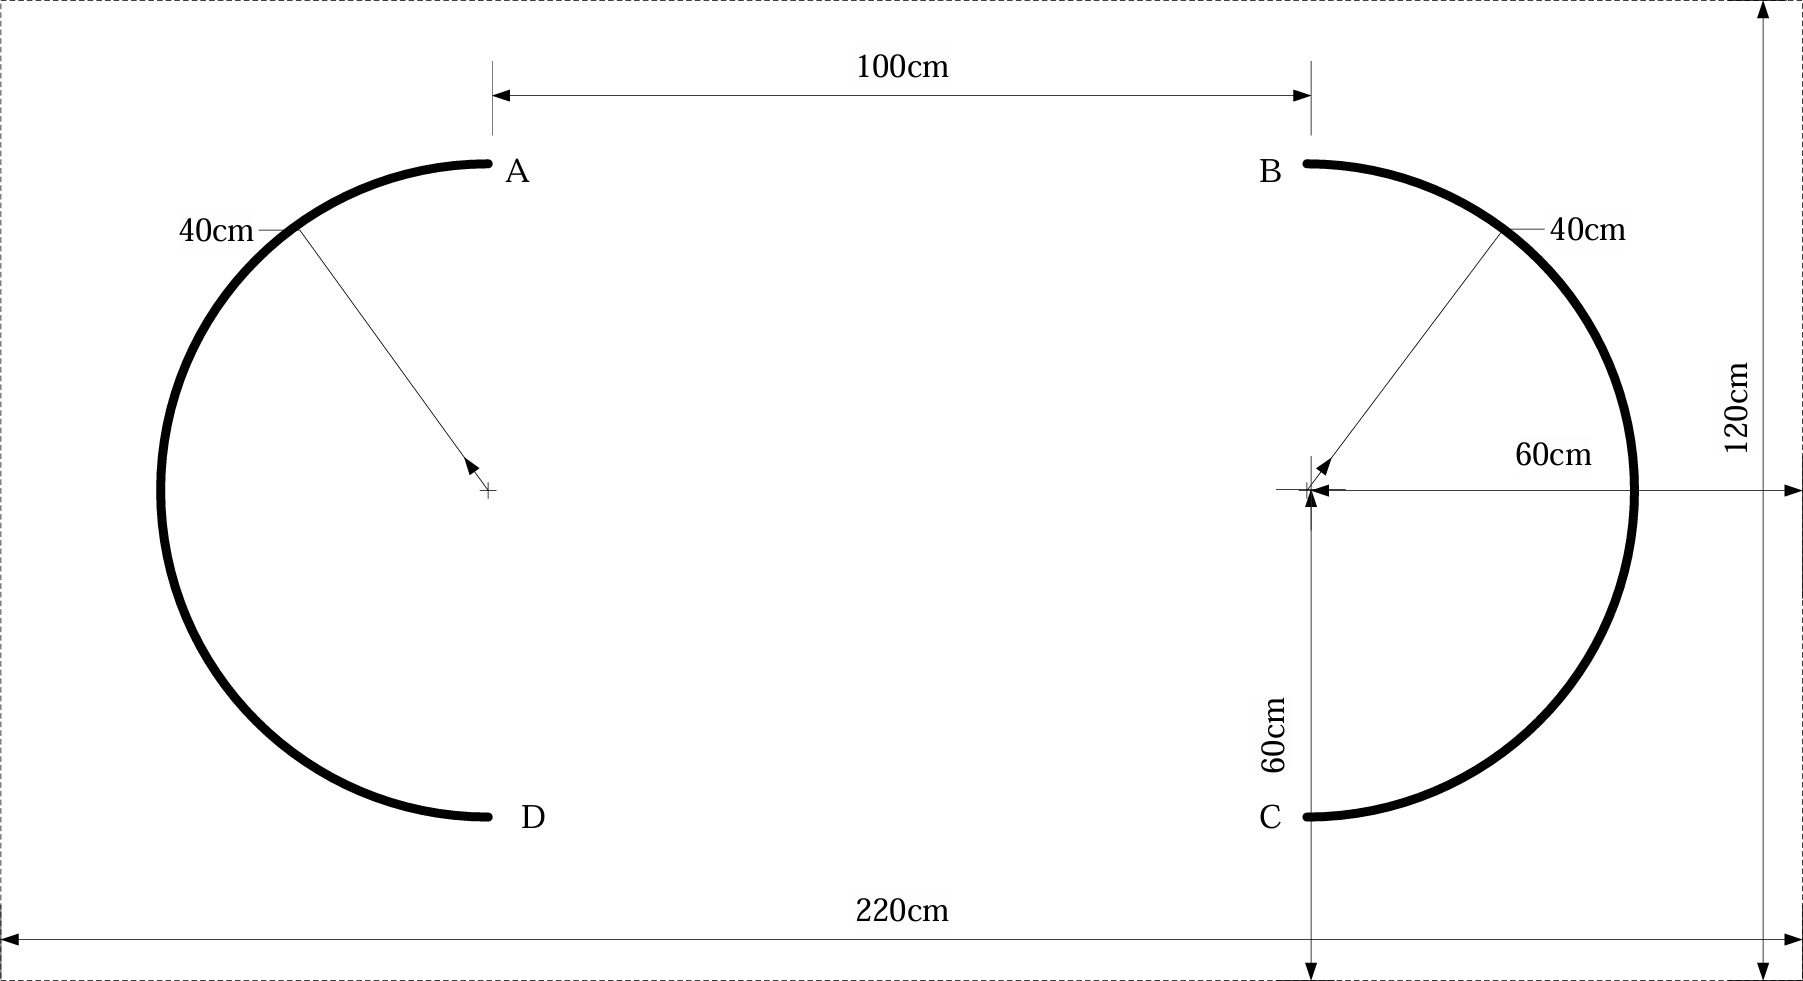
\includegraphics[width=0.88\textwidth]{../../docs_2024/pic1.png}
\caption{H题场地示意图}
\end{figure}

\subsection{功能指标实现方法}
弧线段采用纯追踪模型，将灰度位置偏差 $y$ 转换为曲率 $\kappa$，并据当前线速度 $v$ 计算角速度命令 $\omega$；直线段保持较高基础速度，弧线段根据偏差与黑线覆盖数量自动降速。到达关键点时，任务层通过丢线、航向转角、里程和位姿邻近关系进行确认，并发出声光提示；达到目标圈数后将速度目标清零并保持停车。

\subsection{测量、控制与分析处理}
每个 5\,ms 控制周期中，先读取编码器脉冲并换算车轮速度，再读取 8 路灰度状态、计算线位置与黑线数量；随后依据当前任务状态生成线速度和角速度目标，经差速逆解得到左右轮目标速度，最后由两路增量式 PI 计算 PWM。JY62 数据以 10\,ms 节拍更新，用于航向对齐、直冲段 PD 保持和位姿积分。

\section{核心部件与电路设计}

\subsection{关键器件性能分析}
MSPM0G3507 采用 Cortex-M0+ 内核，可提供定时器、PWM、GPIO 中断和 UART 等资源，满足 200\,Hz 控制与多外设并行需求。TB6612 为双 H 桥电机驱动器，可分别控制左右直流电机的方向与 PWM 占空比。编码器采用 13 线霍尔编码器并配合 30:1 减速比，按 2 倍频计数时每轮一周对应 780 个计数；以轮周长 0.2105\,m 和 200\,Hz 周期可换算实时车速。

\subsection{电路结构工作机理}
电机方向引脚控制 TB6612 的 IN1/IN2 组合，TimerA 输出 10\,kHz PWM，软件将占空比限幅至 0～7800/8000。灰度模块通过地址复用依次选通 8 路检测单元，减少 MCU 引脚占用。编码器 A/B 相上升沿触发 GPIO 中断；JY62 采用 \code{0x55} 帧头、11 字节数据帧解析欧拉角与角速度。电机电源与 MCU 逻辑电源应共地，并在实车接线时复核电流能力和抗干扰措施。

\subsection{运动学与控制模型}
设轮距为 $B$、车体线速度为 $v$、角速度为 $\omega$，则左右轮速度目标为
\begin{equation}
v_L=v-\frac{\omega B}{2},\qquad v_R=v+\frac{\omega B}{2}
\end{equation}
灰度传感器加权位置为
\begin{equation}
y=\frac{\sum(s_i p_i)}{\sum s_i}
\end{equation}
其中 $s_i$ 为第 $i$ 路黑线判定值，$p_i$ 为该传感器横向坐标。纯追踪曲率与角速度命令为
\begin{equation}
\kappa=\frac{2y}{L^2+y^2},\qquad \omega=-K_{\mathrm{steer}}\cdot v\cdot\kappa
\end{equation}
增量式 PI 控制器以 $e(k)=v_{\mathrm{target}}(k)-v_{\mathrm{measured}}(k)$ 为速度偏差：
\begin{equation}
\mathrm{PWM}(k)=\mathrm{PWM}(k-1)+K_p[e(k)-e(k-1)]+K_i e(k)
\end{equation}
本实现中 $K_p=400$、$K_i=300$，PWM 输出限制为 $\pm7800$，以防止控制量超过驱动器有效范围。

\subsection{关键参数与接口}
\begin{table}[H]
\centering
\caption{控制系统关键参数}
\begin{tabularx}{\textwidth}{p{3.2cm}p{3.6cm}Y}
\toprule
参数 & 取值 & 说明\\
\midrule
控制周期 & 5\,ms & TimerG 中断，控制频率 200\,Hz\\
轮距 $B$ & 0.130\,m & 差速运动学参数\\
轮周长 & 0.2105\,m & 编码器速度换算参数\\
编码器计数 & 780/rev & 13线×2倍频×30减速比\\
基础/弯道速度 & 300/185\,mm$\cdot$s$^{-1}$ & 灰度偏差分档速度\\
PWM & 10\,kHz，最大 7800 & TimerA 输出限幅\\
JY62 串口 & 115200\,bps & 航向与角速度数据输入\\
\bottomrule
\end{tabularx}
\end{table}

\section{系统软件设计分析}

\subsection{系统总体工作流程}
上电后完成外设初始化、任务模式选择和传感器状态检查。定时中断中执行“编码器测速→JY62 数据更新→任务状态机→灰度巡线或航向直冲→目标轮速计算→PI 输出→PWM 刷新”流程；主循环负责 OLED 刷新、串口处理、按键及遥测显示。若 IMU 离线，系统不应将航向导航结果视作可用，应降级为循线调试或提示故障。

\subsection{无标记场地的路段状态机}
题目规定场地除两段半圆弧外不得设置额外标记，因此 A、B、C、D 不能通过十字黑线直接识别。软件将任务（3）及任务（4）分解为巡线 A→D、D 点切线对齐、D→B 对角线直冲、巡线 B→C、C 点对齐与前进、C→A 对角线直冲和回到 A 点后的航向恢复等状态。直冲段利用 JY62 的 yaw 与角速度构造 PD 航向保持，检测到黑线后连续确认重捕获，再切换回巡线状态。

\begin{table}[H]
\centering
\caption{T4任务状态机的主要状态}
\begin{tabularx}{\textwidth}{p{2.6cm}p{2.5cm}Yp{2.7cm}}
\toprule
状态 & 输入依据 & 主要动作 & 退出条件\\
\midrule
\code{LINE\_AD} & 灰度线位置、位姿 & 沿 A→D 巡线 & 丢线且接近 D\\
\code{ALIGN\_D} & yaw、角速度 & 对齐 D 点切线及 D→B 航向 & 航向误差连续满足阈值\\
\code{BRIDGE\_D\_TO\_B} & yaw、灰度重捕获 & 按目标航向直冲 & 重捕获黑线\\
\code{LINE\_BC} & 灰度线位置、位姿 & 沿 B→C 巡线 & 丢线且接近 C\\
\code{BRIDGE\_C\_TO\_A} & yaw、灰度重捕获 & 按目标航向直冲 & 重捕获并接近 A\\
\code{STOP} & 圈数计数 & 速度目标清零、声光提示 & 任务结束\\
\bottomrule
\end{tabularx}
\end{table}

\subsection{关键模块程序设计}
灰度模块以传感器横向位置为权重计算 \code{Gray\_Line\_Pos\_mm}，并根据偏差绝对值及黑线数量选择直线、中速或弯道速度。编码器模块完成脉冲计数、速度换算和累计里程；JY62 模块校验帧头与校验和，维护在线超时状态；任务模块统一配置任务（1）至任务（4）的目标圈数与路线。关键接口包括 \code{Gray\_Mode()}、\code{Get\_Target\_Encoder()}、\code{Incremental\_PI\_Left()}、\code{Incremental\_PI\_Right()}、\code{JY62\_GetData()} 与 \code{Gray\_TaskTick()}。

\subsection{可靠性处理}
为抑制单次噪声触发，航向对齐采用连续稳定周期确认；黑线重捕获也采用连续检测计数。对角线直冲设置最大距离与对齐超时保护，避免长期失线。到达已知点后调用位姿快照，将累计积分结果修正为场地坐标，从而降低多圈运行中的漂移。

\section{竞赛工作环境条件}

\subsection{软件环境}
嵌入式程序采用 Keil uVision5 工程进行编译与下载，目标工程为 \code{MSPM0G3507\_Project}；外设配置由 TI SysConfig 生成。调试阶段可使用串口助手、VOFA+ 或 DataScope 观察灰度位置、轮速、航向误差、状态编号和圈数。

\subsection{硬件平台与场地}
硬件平台包括 MSPM0G3507 控制板、TB6612 电机驱动、差速底盘、双路编码器、8 路灰度模块、JY62、OLED、LED、蜂鸣器和车载电池。测试场地按题目制作，面积不小于 220\,cm×120\,cm，半圆弧半径 40\,cm、线宽约 1.8\,cm，场地上不得添加用于辅助导航的标记。

\subsection{调试条件与安全事项}
先在架空状态确认左右轮方向、PWM 极性、编码器计数符号和急停逻辑，再在低速下完成灰度阈值、传感器安装位置与纯追踪增益整定。电机电源应满足峰值电流需求；调试期间避免车轮被障碍物卡死，并在改动供电或接线后重新验证共地与极性。

\section{作品成效总结分析}

\subsection{测试方案}
按由简到难的顺序验证：首先进行 A→B 单弧线测试，确认巡线、端点判断与停车；其次完成任务（2）单圈，检查四段衔接与声光提示；再完成任务（3）逆向路线，检查对角线直冲、航向对齐和重捕获；最后进行任务（4）四圈连续运行，统计总用时、单圈波动、成功率、停车误差和失线恢复次数。每组条件至少重复 3 次，并记录电池电压和场地状态。

\begin{table}[H]
\centering
\caption{实车测试记录表（须由调试数据补录）}
\small
\begin{tabularx}{\textwidth}{p{2.1cm}Yp{1.25cm}p{1.25cm}p{1.25cm}p{1.35cm}}
\toprule
测试项目 & 评价指标 & 第1次 & 第2次 & 第3次 & 结论\\
\midrule
任务（1）A→B & 用时$\leq15$\,s、停车与声光提示 & 待实测 & 待实测 & 待实测 & 待判定\\
任务（2）单圈 & 用时$\leq30$\,s、各点提示 & 待实测 & 待实测 & 待实测 & 待判定\\
任务（3）单圈 & 用时$\leq40$\,s、路径正确 & 待实测 & 待实测 & 待实测 & 待判定\\
任务（4）四圈 & 总用时、连续完成率 & 待实测 & 待实测 & 待实测 & 待判定\\
\bottomrule
\end{tabularx}
\end{table}

\subsection{成效与不足分析}
从软件实现角度看，系统已将基础灰度巡线、编码器速度闭环、IMU 航向保持与 T4 状态机集成在统一控制框架中，能够针对无额外标记的场地建立可解释的过点与重捕获逻辑。该方案的优势是计算量低、模块边界清晰，并允许按任务切换目标圈数。其局限在于灰度特征会受传感器高度、环境光和线宽影响，里程计受轮胎打滑影响，IMU 存在零偏与航向漂移；因此最终性能必须以本章实测数据为准，并根据实车日志迭代阈值与增益。

\subsection{创新特色与展望}
本设计以“循线优先、惯导补偿、已知点校正”的分层方式完成复杂路段控制：正常情况下由低成本灰度阵列完成闭环循迹，失线或跨越路段由 IMU 保持航向，重回已知点后以位姿快照抑制误差累积。后续可基于黑匣子遥测记录分析误差分布，采用自适应速度规划、灰度阈值在线校准和航向零偏补偿，提高不同场地和电池状态下的重复性。

\section{参考资料及文献}
\begin{enumerate}[label={[\arabic*]}]
  \item 2024年全国大学生电子设计竞赛江苏赛区（TI杯）自动行驶小车（H题）试题。
  \item 项目资料：H题路线分解与代码适配，\code{docs\_2024/H题路线分解.md}。
  \item 项目资料：H题核心算法详解，\code{docs\_2024/H题算法详解.md}。
  \item Texas Instruments. \textit{MSPM0G3507 Microcontrollers Technical Reference Manual}.
  \item JY62 使用说明书：串口姿态数据帧与角速度数据格式。
\end{enumerate}

\section{附件材料}
\subsection{工程文件与关键源代码}
工程文件位于 \code{firmware/WHEELTEC\_C07A\_CAR\_JY62\_GapBridge/}。其中 \code{Control/control.c} 实现 5\,ms 控制中断、灰度循迹、T4 位姿导航与速度闭环；\code{Hardware/jy62.c} 实现姿态数据帧解析；\code{Hardware/motor.c}、\code{encoder.c} 与 \code{CCD.c} 分别实现电机、编码器和灰度外设驱动。

\subsection{最终提交前检查清单}
\begin{itemize}
  \item[$\square$] 核对 MCU 型号、车体尺寸、前进限制和无摄像头要求。
  \item[$\square$] 补录全部实测数据、测试视频编号及异常现象。
  \item[$\square$] 核验声光提示、最终停车位置及连续四圈完成情况。
  \item[$\square$] 复查电源容量、接线可靠性和现场光照下的传感器阈值。
\end{itemize}

\end{document}
